\chapter{Arhitektura i dizajn sustava}
		
Da bismo razradili arhitekturu web aplikacije za poboljšanje dostupnosti knjiga prevedenih na hrvatski i srodne jezike, detaljnije ćemo opisati njene komponente, organizaciju i međusobnu komunikaciju. Evo ključnih elemenata:
	\\
	
	\section{Komponente}

        \subsubsection{Stil arhitekture}
        Stil arhitekture bi mogao biti mikroservisni ili slojeviti (npr. MVC - Model-View-Controller). Mikroservisni pristup omogućava modularnost i lako skaliranje, dok slojeviti pristup olakšava razvoj i održavanje. Prilikom razvoja naše aplikacije odabran je MVC model.
        
        
        \subsubsection{Podsustavi}

        Podsustavi se mogu podijeliti na:
        \begin{itemize}
		  \item {Korisničko sučelje (UI): Front-end komponenta zadužena za interakciju s korisnicima.}
		  \item {Poslovna logika: Središnji dio koji upravlja funkcionalnostima aplikacije.}
		  \item {Baza podataka: Spremište podataka gdje se čuvaju informacije o knjigama, korisnicima, ponuditeljima, itd.}		
            \item {Autentikacija i autorizacija: Sustav za upravljanje korisničkim pristupima i ovlastima.}	
             \item {Integracija vanjskih usluga: Za funkcionalnosti poput prikaza karte (npr. integracija OpenStreetMap).}		
	   \end{itemize}

        \subsubsection{Preslikavanje na radnu platformu}

        Komponente se raspoređuju na servere i klijentske uređaje:
        \begin{itemize}
		  \item {Server: Hostira poslovnu logiku, bazu podataka, autentikaciju i API za integraciju vanjskih usluga.}
		  \item {Klijent: Uređaji korisnika (mobiteli, tableti, računala) s web preglednikom za pristup UI.}
	   \end{itemize}
    
    \subsubsection{Spremišta podataka}

        Centralizirana baza podataka (SQL ili NoSQL) koja pohranjuje:
        \begin{itemize}
		  \item {Podatke o knjigama.}
		  \item {Informacije o korisnicima i ponuditeljima.}
		  \item {Zahtjeve za prijevod i ponude.}				
	   \end{itemize}

    \subsubsection{Mrežni protokoli}
    
    \begin{itemize}
		  \item {HTTP/HTTPS: Za komunikaciju između klijenta i servera.}
		  \item {API protokoli (REST, GraphQL): Za upite i manipulaciju podacima.}
	   \end{itemize}

    \subsubsection{Globalni upravljački token}

        Sustav bi koristio zahtjev-odgovor model za komunikaciju između klijenta i servera. Autentikacija i autorizacija korisnika odvijaju se na početku sesije.
    
    \subsubsection{Sklopovsko-programski zahtjevi}

    \begin{itemize}
		  \item {Server: Pouzdan i skalabilan, s dovoljno resursa za obradu zahtjeva i pohranu podataka.}
		  \item {Klijent: Kompatibilnost s modernim web preglednicima i prilagodljivost različitim veličinama ekrana.}			
	   \end{itemize}
	   
	   
	   \begin{itemize}
	   	\item {Prikazuje raspored glavnih komponenti: UI, poslovna logika, baza podataka, autentikacija.}
	   	\item {Ilustrira komunikaciju između klijenta i servera.}			
	   \end{itemize}
	   
		
		\eject
		
		\begin{figure}[H]
			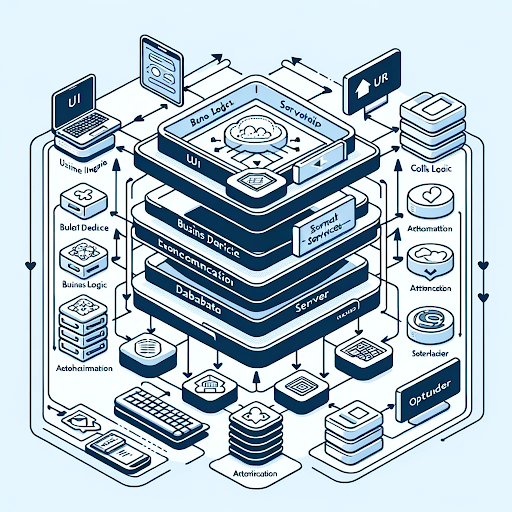
\includegraphics[width=\textwidth]{slike/arhitektura.PNG} %veličina u odnosu na širinu linije
			\centering
			\caption{Osnova arhitekture}
			\label{fig5:promjene}
		\end{figure}
		
		\eject
	
  Skica ilustrira sljedeće komponente i njihovu međusobnu komunikaciju:
   \begin{itemize}
		  \item {Korisničko sučelje (UI): Na klijentskim uređajima (mobitel, tablet, računalo).}
		  \item {Poslovna logika: Dio koji se nalazi na serveru.}	
            \item {Baza podataka: Spremište podataka također na serveru.}
		  \item {Autentikacija: Dio za upravljanje korisničkim pristupom.}	
            \item {Integracija vanjskih usluga: Na primjer, OpenStreetMap za prikaz karata.}
	   \end{itemize}

Izbor Model-View-Controller (MVC) arhitekture za ovu web aplikaciju temelji se na nekoliko ključnih principa oblikovanja koje sam uzimao u obzir:

	\eject
	
	\section{Izbor arhitekture}

 	\subsubsection{Separacija briga (Separation of concerns)}

MVC arhitektura odlično odvaja različite aspekte aplikacije:
\begin{itemize}
		  \item {Model: Predstavlja podatke i poslovnu logiku aplikacije. U ovom slučaju, model bi upravljao podacima knjiga, korisnika, ponuda i zahtjeva za prijevod.}
		  \item {View: Odnosi se na korisničko sučelje. U našoj aplikaciji, ovo bi bilo mjesto gdje korisnici pretražuju knjige, pregledavaju ponude, i komuniciraju sa sustavom.}	
            \item {Controller: Djeluje kao posrednik između Modela i Viewa, obrađuje korisničke zahtjeve, ažurira model i konačno šalje podatke natrag viewu.}
	   \end{itemize}

Ova jasna podjela pomaže u organizaciji koda, olakšava održavanje i omogućava lakše testiranje pojedinih komponenti.
	\\

 \subsubsection{Skalabilnost i fleksibilnost}

MVC podržava skalabilnost. Kako se aplikacija razvija, svaki dio (Model, View, Controller) može se neovisno skalirati ili modificirati. Ovo je posebno korisno za aplikacije koje imaju potencijal rasti, kao što je naš slučaj s web platformom za knjige.
	\\

 \subsubsection{Podrška za više klijentskih platformi}

S obzirom na to da se aplikacija mora prilagoditi različitim uređajima (mobilnim telefonima, tabletima, računalima), MVC omogućava razvoj različitih vrsta viewova koji mogu koristiti isti model i controller logiku. To znači da možemo imati različite korisničke sučelja za mobilne uređaje i desktop računala, dok se poslovna logika i obrada podataka ne mijenjaju.
	\\

 \subsubsection{Održavanje i nadogradnja}

MVC struktura pojednostavljuje ažuriranja i održavanje. Ako trebate promijeniti poslovnu logiku, to se može učiniti u modelu bez utjecaja na view. Slično, izmjene u korisničkom sučelju ne utječu na poslovnu logiku aplikacije.
	\\
	
 \subsubsection{Zajednica i resursi}

MVC je popularan i dobro dokumentiran arhitekturni obrazac. Postoji obilje resursa, biblioteka i okvira koji podržavaju MVC, što može značajno ubrzati razvoj i pružiti bolju podršku tijekom razvojnog procesa.

Zbog ovih razloga, MVC se čini kao optimalan izbor za arhitekturu ove web aplikacije, pružajući dobru osnovu za jasno strukturiran, održiv i fleksibilan razvoj.


Organizacija sustava za opisanu web aplikaciju s najviše razine apstrakcije može se podijeliti u četiri glavne komponente: klijent-poslužitelj model, baza podataka, datotečni sustav, i grafičko sučelje. Ove komponente zajedno omogućavaju funkcionalnost, skalabilnost i korisničku interakciju potrebnu za uspješan rad aplikacije.

	\eject
	
	\section{Organizacija sustava}

 \subsubsection{Klijent-poslužitelj model}

U klijent-poslužitelj modelu, aplikacija je podijeljena na dva glavna dijela: klijent (front-end) koji se izvodi na korisničkom uređaju i poslužitelj (back-end) koji obrađuje zahtjeve i šalje odgovore.
\begin{itemize}
		  \item {Klijent (Front-end): Koristi web preglednik ili mobilnu aplikaciju za pristup aplikaciji. Odgovoran je za prikupljanje korisničkih ulaza, prikazivanje podataka korisnicima i slanje zahtjeva poslužitelju.}
		  \item {Poslužitelj (Back-end): Hostira aplikaciju, obrađuje zahtjeve, vrši operacije nad bazom podataka, i vraća rezultate klijentu. Također upravlja autentikacijom, autorizacijom, i sigurnošću.}	\\
	   \end{itemize}
	   


 \subsubsection{Baza podataka}

Baza podataka je središnje mjesto za pohranu svih podataka koji su relevantni za aplikaciju. Uključuje:
\begin{itemize}
		  \item {Podatke o knjigama: Nazive, autore, žanrove, godine izdanja, itd.}
		  \item {Korisničke podatke: Informacije o registriranim i neregistriranim korisnicima.}	
            \item {Ponude i zahtjeve: Informacije o dostupnosti knjiga, ponuditeljima, i zahtjevima za prijevod.} \\
	   \end{itemize} 


 \subsubsection{Datotečni sustav}

Datotečni sustav se koristi za pohranu i upravljanje datotekama koje nisu direktno povezane s bazom podataka, poput:
\begin{itemize}
		  \item {Slika korica knjiga: Pohranjene kao datoteke koje se mogu prikazivati u korisničkom sučelju.}
		  \item {Dokumenti: Uključujući priručnike, upute za korisnike, i druge dokumente.} \\
	   \end{itemize} 

 \subsubsection{Grafičko sučelje}

Grafičko sučelje (GUI) je ono što korisnik vidi i s čime interagira. Uključuje:
\begin{itemize}
		  \item {Web stranice: Dizajnirane za jednostavno korištenje i navigaciju, s funkcionalnostima kao što su pretraga, pregled knjiga, i slanje zahtjeva.}
		  \item {Mobilno sučelje: Prilagođeno za manje ekrane i osjetljivo na dodir, s sličnim funkcionalnostima kao web verzija.}	\\
	   \end{itemize} 

Svaka od ovih komponenti igra ključnu ulogu u uspješnom funkcioniranju aplikacije, omogućujući efikasnu obradu podataka, intuitivnu korisničku interakciju i sigurnost informacija.

\eject

\section{Organizacija aplikacije}

Organizacija aplikacije koja koristi Model-View-Controller (MVC) arhitekturu s jasno definiranim frontend i backend slojevima omogućava efikasno upravljanje kodom i funkcionalnostima. Evo kako bi se to moglo strukturirati:

 \subsubsection{Frontend (klijentska strana)}

Frontend je ono što korisnik vidi i s čime interagira. U MVC arhitekturi, to uglavnom obuhvaća "View" komponentu.
\begin{itemize}
		  \item {Tehnologije: HTML, CSS, JavaScript, i frameworki poput React, Angular ili Vue.js.}
		  \item {Zadaće:
    \begin{itemize}
		  \item {Prikaz podataka: Dinamički prikazuje podatke dobivene s backend-a.}
		  \item {Korisničko sučelje: Omogućava interakciju s korisnikom, prikuplja korisničke zahtjeve i šalje ih backend-u.}	
            \item {Odgovor na korisničke akcije: Ažuriranje sučelja na temelju korisničkih interakcija i podataka s backend-a.} \\
	   \end{itemize}}	
            
	   \end{itemize}


 \subsubsection{Backend (poslužiteljska strana)}

Backend se bavi obradom podataka, poslovnom logikom i interakcijom s bazom podataka. U MVC arhitekturi, to uključuje "Model" i "Controller" komponente.
\begin{itemize}
		  \item {Tehnologije: Server-side jezici poput Node.js, Python (Django, Flask), Ruby on Rails, Java (Spring), itd.}
		  \item { Zadaće:
            \begin{itemize}
		  \item { Controller:
                    \begin{itemize}
		  \item {Upravlja zahtjevima s frontend-a.}
		  \item {Prosljeđuje podatke između View-a i Modela.}	
            \item {Upravlja tokom podataka i obradi zahtjeva.}
	   \end{itemize}}
        \item { Model:
                    \begin{itemize}
		  \item {Predstavlja poslovnu logiku i podatke.}
		  \item {Interakcija s bazom podataka.}	
            \item {Obrada podataka (CRUD operacije - Create, Read, Update, Delete).} \\
	   \end{itemize}}
	   \end{itemize}}	
	   \end{itemize}


 \subsubsection{Komunikacija između frontend-a i backend-a}

Komunikacija između frontend-a i backend-a obično se odvija preko API-ja (Application Programming Interface), koristeći HTTP/HTTPS protokole.
\begin{itemize}
		  \item {API (najčešće REST ili GraphQL): Definira kako frontend šalje zahtjeve backend-u i kako backend vraća odgovore.}
		  \item {JSON format: Često korišten format za slanje podataka između frontend-a i backend-a.}	\\
	   \end{itemize}


 \subsubsection{Baza podataka}

Iako tehnički nije dio MVC strukture, baza podataka je ključna komponenta koja surađuje s Modelom. Ona pohranjuje sve podatke potrebne za aplikaciju.
\begin{itemize}
		  \item {Tehnologije: SQL (MySQL, PostgreSQL) ili NoSQL (MongoDB, Cassandra) baze podataka.}
		  \item {Zadaće: Pohrana i dohvaćanje podataka potrebnih za aplikaciju.}	
	   \end{itemize}

U ovakvoj organizaciji, svaki sloj ima jasno definiranu ulogu, što doprinosi boljem razumijevanju koda, lakšem održavanju i skaliranju aplikacije. Frontend i backend mogu se neovisno razvijati i optimizirati, što pruža fleksibilnost i efikasnost u razvojnom procesu.

\eject

				
		\section{Baza podataka}
		
		
			\subsection{Opis tablica}
				
				
				\begin{longtblr}[
					label=none,
					entry=none
					]{
						width = \textwidth,
						colspec={|X[8,l]|X[8, l]|X[20, l]|}, 
						rowhead = 1,
					} %definicija širine tablice, širine stupaca, poravnanje i broja redaka naslova tablice
					
					\hline \SetCell[c=3]{c}{\textbf{Korisnik}}	 \\ \hline[3pt]
					\SetCell{LightBlue} & VARCHAR(13) & \\ \hline
					userId & INT & Jedinstveni identifikator, autogeneriran od strane baze \\ \hline
					username & VARCHAR & Jedinstveno korisničko ime \\ \hline
					password & VARCHAR & Jedinstveno lozinka \\ \hline
					naziv & VARCHAR & Naziv korisnika \\ \hline
					adresa & VARCHAR & Adresa korisnika \\ \hline
					telefon & INT & Telefon korisnika \\ \hline
					email & VARCHAR & Email korisnika \\ \hline
					tip & VARCHAR & Tip korisnika \\ \hline
					\\
					
					\hline \SetCell[c=3]{c}{\textbf{Knjiga}}	 \\ \hline[3pt]
					\SetCell{LightGreen} & VARCHAR(13) & \\ \hline
					bookId & INT & Jedinstveni identifikator, autogeneriran od strane baze \\ \hline
					naslov	& VARCHAR & Naziv knjige \\ \hline 
					autor & VARCHAR & Ime autora \\ \hline 
					izdavač & VARCHAR & Ime izdavača	\\ \hline
					brojIzdanja & INT & Broj izdanja knjige	\\ \hline 
					godIzdanja & INT & Godina izdanja knjige	\\ \hline
					kategorija & CHAR(3) & Kategorija izdavača	\\ \hline
					zahtjevi & INT & Zahtjev za prijevod knjige	\\ \hline
					očuvanost & VARCHAR & Očuvanost knjige	\\ \hline
					opis & VARCHAR & Kratki opis knjige	\\ \hline
					slika & VARCHAR & Prikaz knjige	\\ \hline
					žanr & VARCHAR & Žanr knjige \\ \hline
					isbn & INT & ISBN knjige \\ \hline
					\\
					
					\hline \SetCell[c=3]{c}{\textbf{Ponuda}}	 \\ \hline[3pt]
					\SetCell{LightGreen} & VARCHAR(32) & \\ \hline
					offerId	& INT & Jedinstveni identifikator, autogeneriran od strane baze  	\\ \hline 
					nazivPonuditelja & VARCHAR & Naziv ponuditelja  \\ \hline 
					brojPrimjeraka & INT & Broj primjeraka knjige 		\\ \hline 
					cijena & INT & Cijena knjige \\	\hline
					\\
					
			   \end{longtblr}
				
				
			
			\subsection{Dijagram baze podataka} 
				
				\begin{figure}[H]
					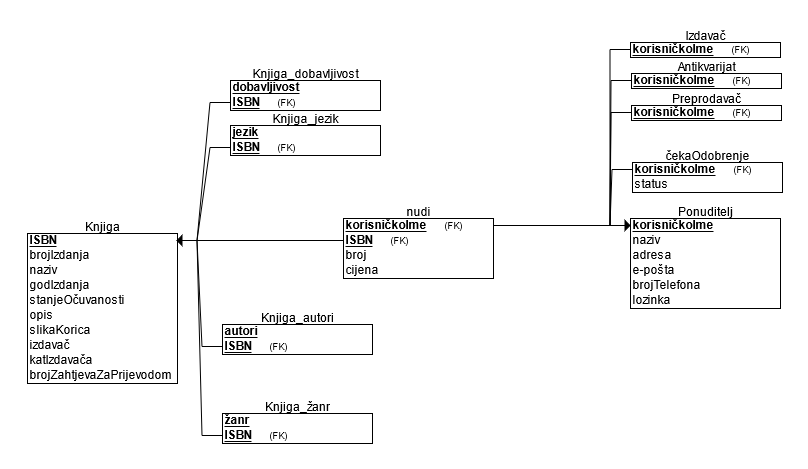
\includegraphics[width=\textwidth]{dijagrami/baza_relmod_v2.PNG} %veličina u odnosu na širinu linije
					\centering
					\caption{REL dijagram baze podataka}
					\label{fig:arh1}
				\end{figure}
				
				\eject
				
				\begin{figure}[H]
					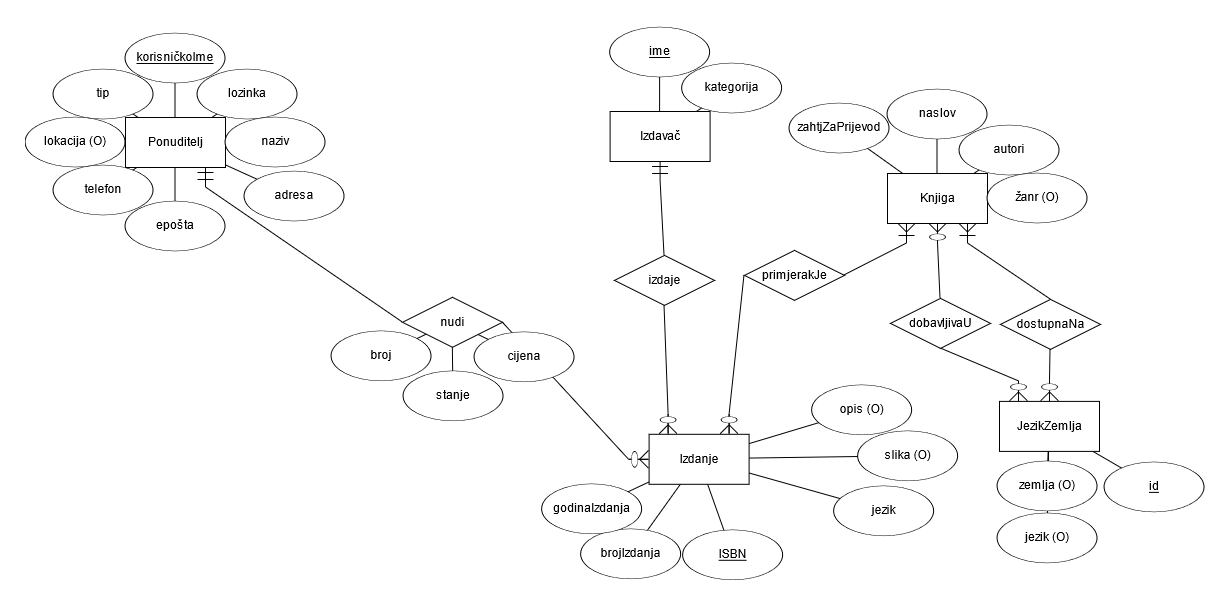
\includegraphics[width=\textwidth]{dijagrami/baza_ERmod_v3.PNG} %veličina u odnosu na širinu linije
					\centering
					\caption{ER dijagram baze podataka}
					\label{fig:arh2}
				\end{figure}
				
			
			\eject
			
			
		\section{Dijagram razreda} 
			
			Idejno razrađeni dijagram razreda opisuje strukturu web aplikacije. Uključuje ApplicationController za upravljanje zahtjevima vezanim uz navigaciju na web stranici, KorisnikController za obrađivanje korisničkih zahtjeva, LoginController za autentikaciju korisnika te Korisnik za predstavljanje entiteta korisnika. KorisnikService brine o logici poslovne logike vezane uz korisnike, dok KorisnikRepository predstavlja sučelje za pristup podacima korisnika u bazi podataka. StoZelisCitatiApplication predstavlja glavni razred aplikacije s main metodom za pokretanje, dok su veze između razreda usmjerene prema ovisnostima i suradnji između njih. Ovo omogućava bolje razumijevanje strukture aplikacije, odvojenost odgovornosti i međusobnu interakciju između komponenti. \\ \\
			
			\begin{figure}[H]
				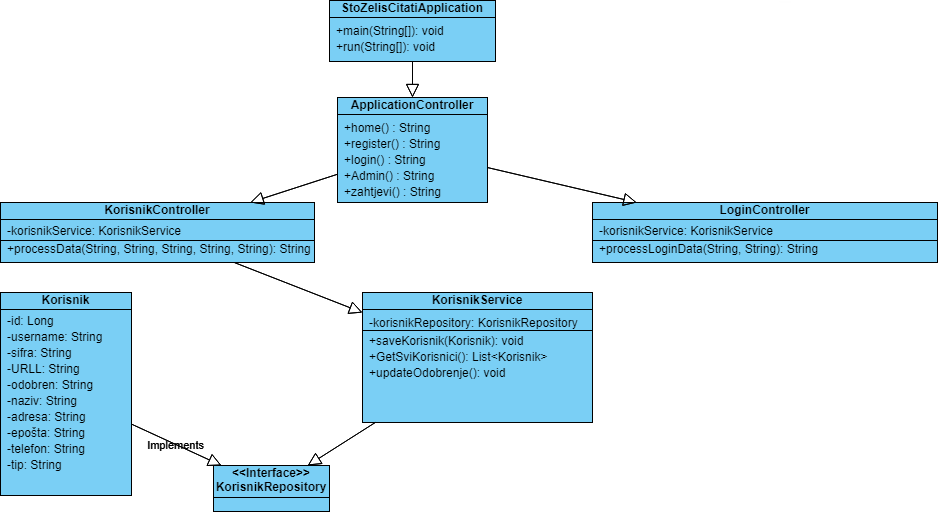
\includegraphics[width=\textwidth]{dijagrami/ClassDiagram1.PNG} %veličina u odnosu na širinu linije
				\centering
				\caption{Dijagram razreda}
				\label{fig:razred}
			\end{figure}
			
			\eject
			
			
			Idejno razrađeni dijagram razreda opisuje sve tri vrste ponuditelja te njihove funkcionalnosti. Predstavljena je ovisnost i suradnja između razreda.
			\\ \\
			
				\begin{figure}[H]
				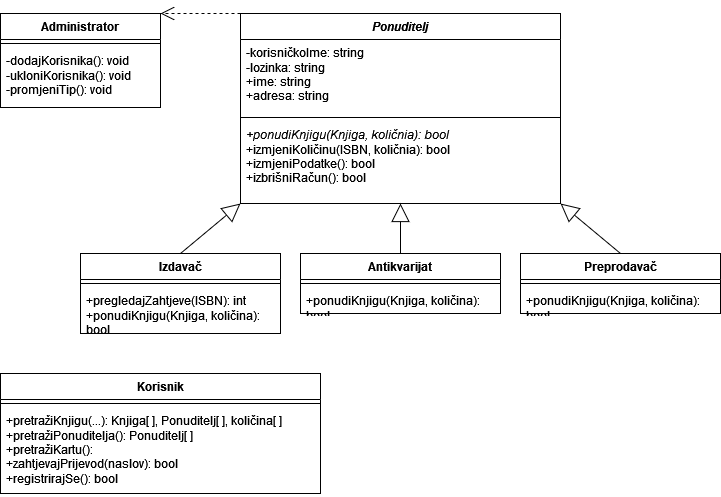
\includegraphics[width=\textwidth]{dijagrami/UML dijagram razreda v1.PNG} %veličina u odnosu na širinu linije
				\centering
				\caption{Dijagram razreda}
				\label{fig:razred1}
			\end{figure}
			
			\eject
			
						
			
			
			\begin{figure}[H]
				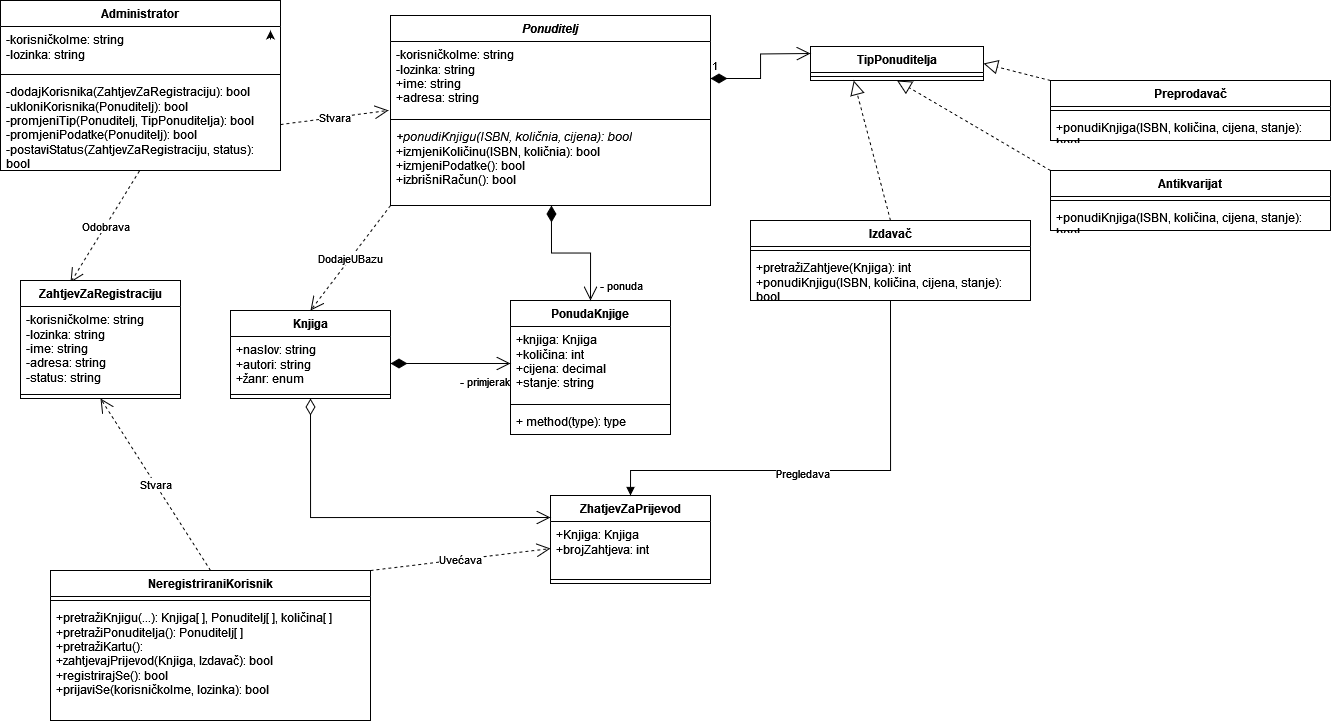
\includegraphics[width=\textwidth]{dijagrami/UML dijagram razreda v2.PNG} %veličina u odnosu na širinu linije
				\centering
				\caption{Dijagram razreda}
				\label{fig:razred2}
			\end{figure}
			
			
			\eject
		
		\section{Dijagram stanja}
			
			
			Dijagram stanja se koristi za modeliranje ponašanja sustava ili entiteta s obzirom na različita stanja kroz koje može proći. Sadrži stanja, prijelaze između stanja, događaje koji pokreću prijelaze te akcije koje se izvršavaju u svakom stanju ili prijelazu. Na slici je prikazan dijagram stanja za registriranog korisnika. Nakon uspješne prijave, korisniku se prikazuje početna stranica na kojoj može vidjeti svoje ponude knjiga te napraviti novu ponudu knjige. Za odabranu knjigu potrebno je provjeriti treba li zatražiti prijevod iste ili ne te zatim unijeti potrebne podatke i zaključiti ponudu. Korisniku se klikom na "Osobni podaci" prikazuju njegovi podaci koje može urediti, a klikom na "Moje ponude" može pregledati sve svoje ponude knjiga.
			
			\eject
			
			
			\begin{figure}[H]
				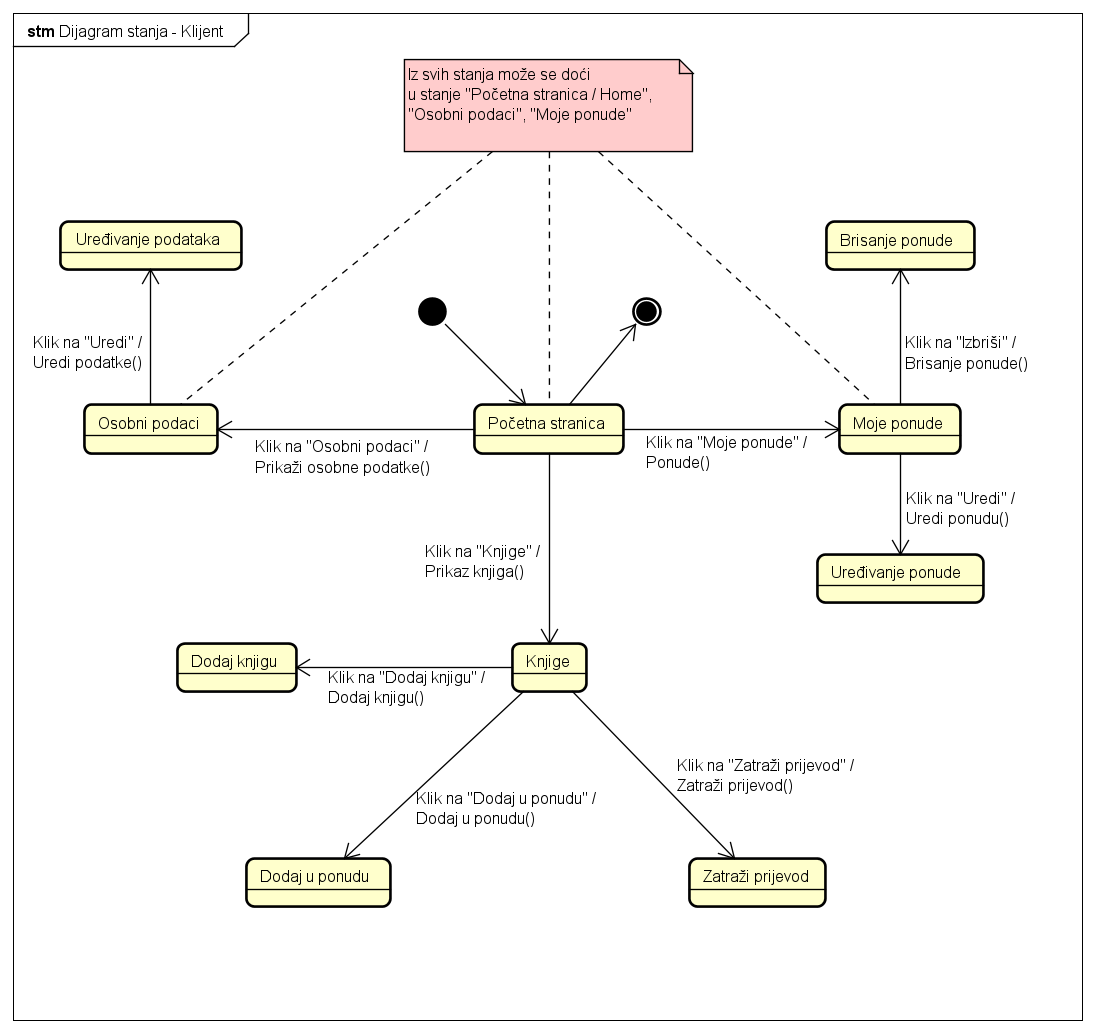
\includegraphics[width=\textwidth]{dijagrami/Dijagram stanja.PNG} %veličina u odnosu na širinu linije
				\centering
				\caption{Dijagram stanja }
				\label{fig:dijagramstanja1}
			\end{figure} 
			
			
			\eject 
		
		\section{Dijagram aktivnosti}
			
			
			Dijagram aktivnosti se koristi za modeliranje poslovnih procesa, algoritama ili drugih sekvenci aktivnosti unutar sustava što je vrlo korisno za opisivanje tokova rada ili procesa izvođenja zadataka. Sadrži stanja, aktivnosti, odluke, ulazne i izlazne tokove te usklađivačke elemente koji pomažu u opisu redoslijeda aktivnosti. Na sljedećem dijagramu prikazan je proces kreiranja nove ponude knjige. Korisnik, nakon prijave u sustav te odobravanja iste, odabire knjigu koju želi dodati u ponudu. Također će zatražiti zahtjev za prijevod ako je to potrebno.
			Nakon unosa svih potrebnih podataka, korisnik zaključuje ponudu. 
			
			\eject
			
			
			\begin{figure}[H]
				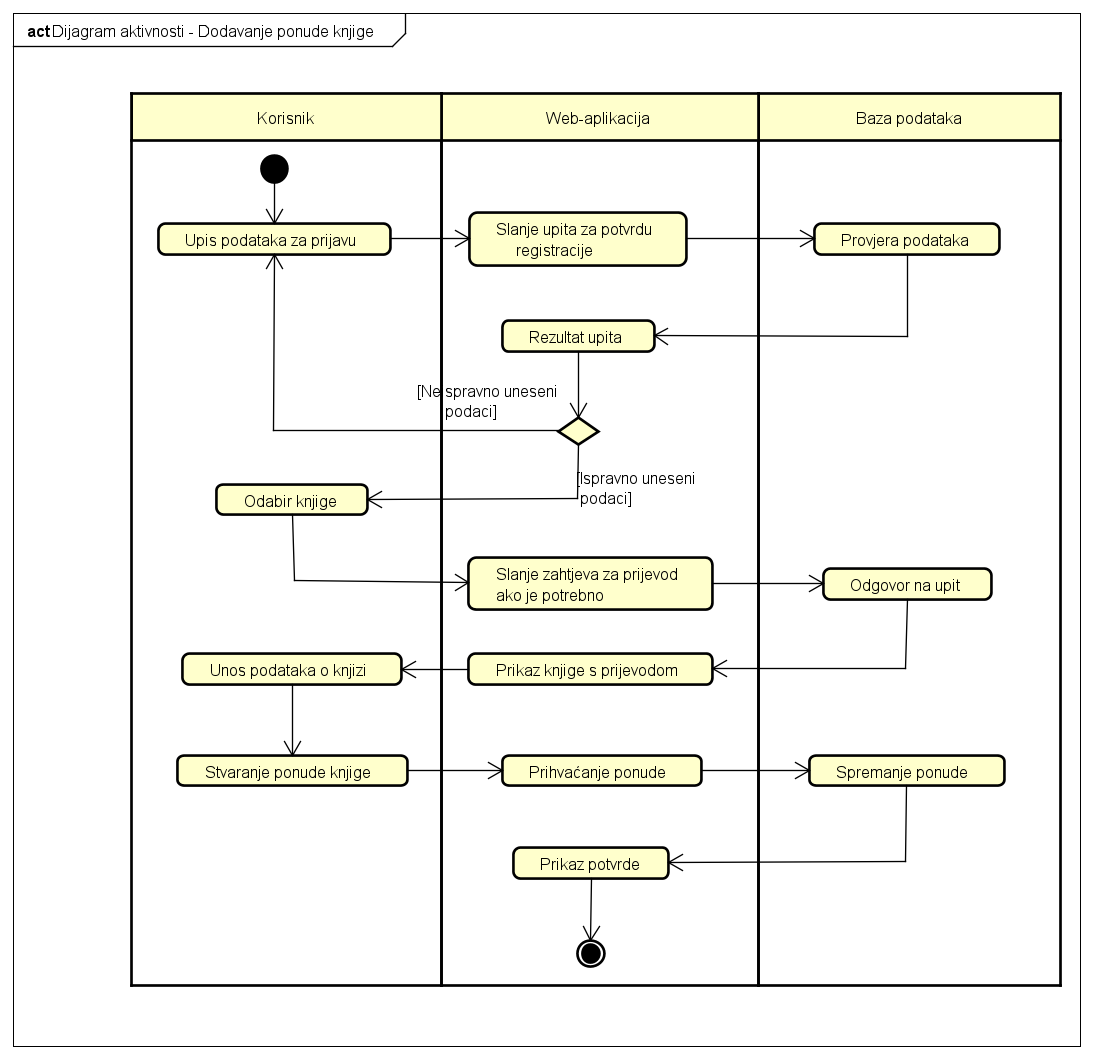
\includegraphics[width=\textwidth]{dijagrami/Dijagram aktivnosti.PNG} %veličina u odnosu na širinu linije
				\centering
				\caption{Dijagram aktivnosti }
				\label{fig:dijagramaktivnosti1}
			\end{figure}
			
			\eject
			
		\section{Dijagram komponenti}
		
			Dijagram komponenti je vrsta strukturnog dijagrama koja prikazuje logičke komponente sustava i njihove odnose. Na ovom dijagramu su vdiljive komponente Prijava, Pretraživanje, Prikaz karte i Prikaz registriranog korisnika koje djeluju unutar React view komponente unutar Frontend web prikaza komponente. One su preko sučelja za dohvat HTML, CSS i JS povezane s komponentom Main.JSX koja funkcionira kao router koji upravlja prikazom i funkcionalnošću grafičkog prikaza. Ovisno o potrebi upravlja ih na komponente AdminPage, RegisterPage, LoginPage, UserPage, BookPage, OfferPage, te HomePage. Sve te komponente se nalaze u Web aplikaciji. Dodatno u Web aplikaciji je komponenta REST API koja je povezana s komponentama za pretraživanje i prikaz registriranog korisnika preko sučelja dohvat JSON. Ona ovisno o potrebi se nadovezuje na Prikaz ponude knjiga koja je preko sučelja SQL povezana s vanjskom komponentom Baza podataka. Ili Prikaz karte koja je preko sučelja REACT API povezana s vanjskom komponento OpenStreetMap. 

            \eject
			
			
			\begin{figure}[H]
				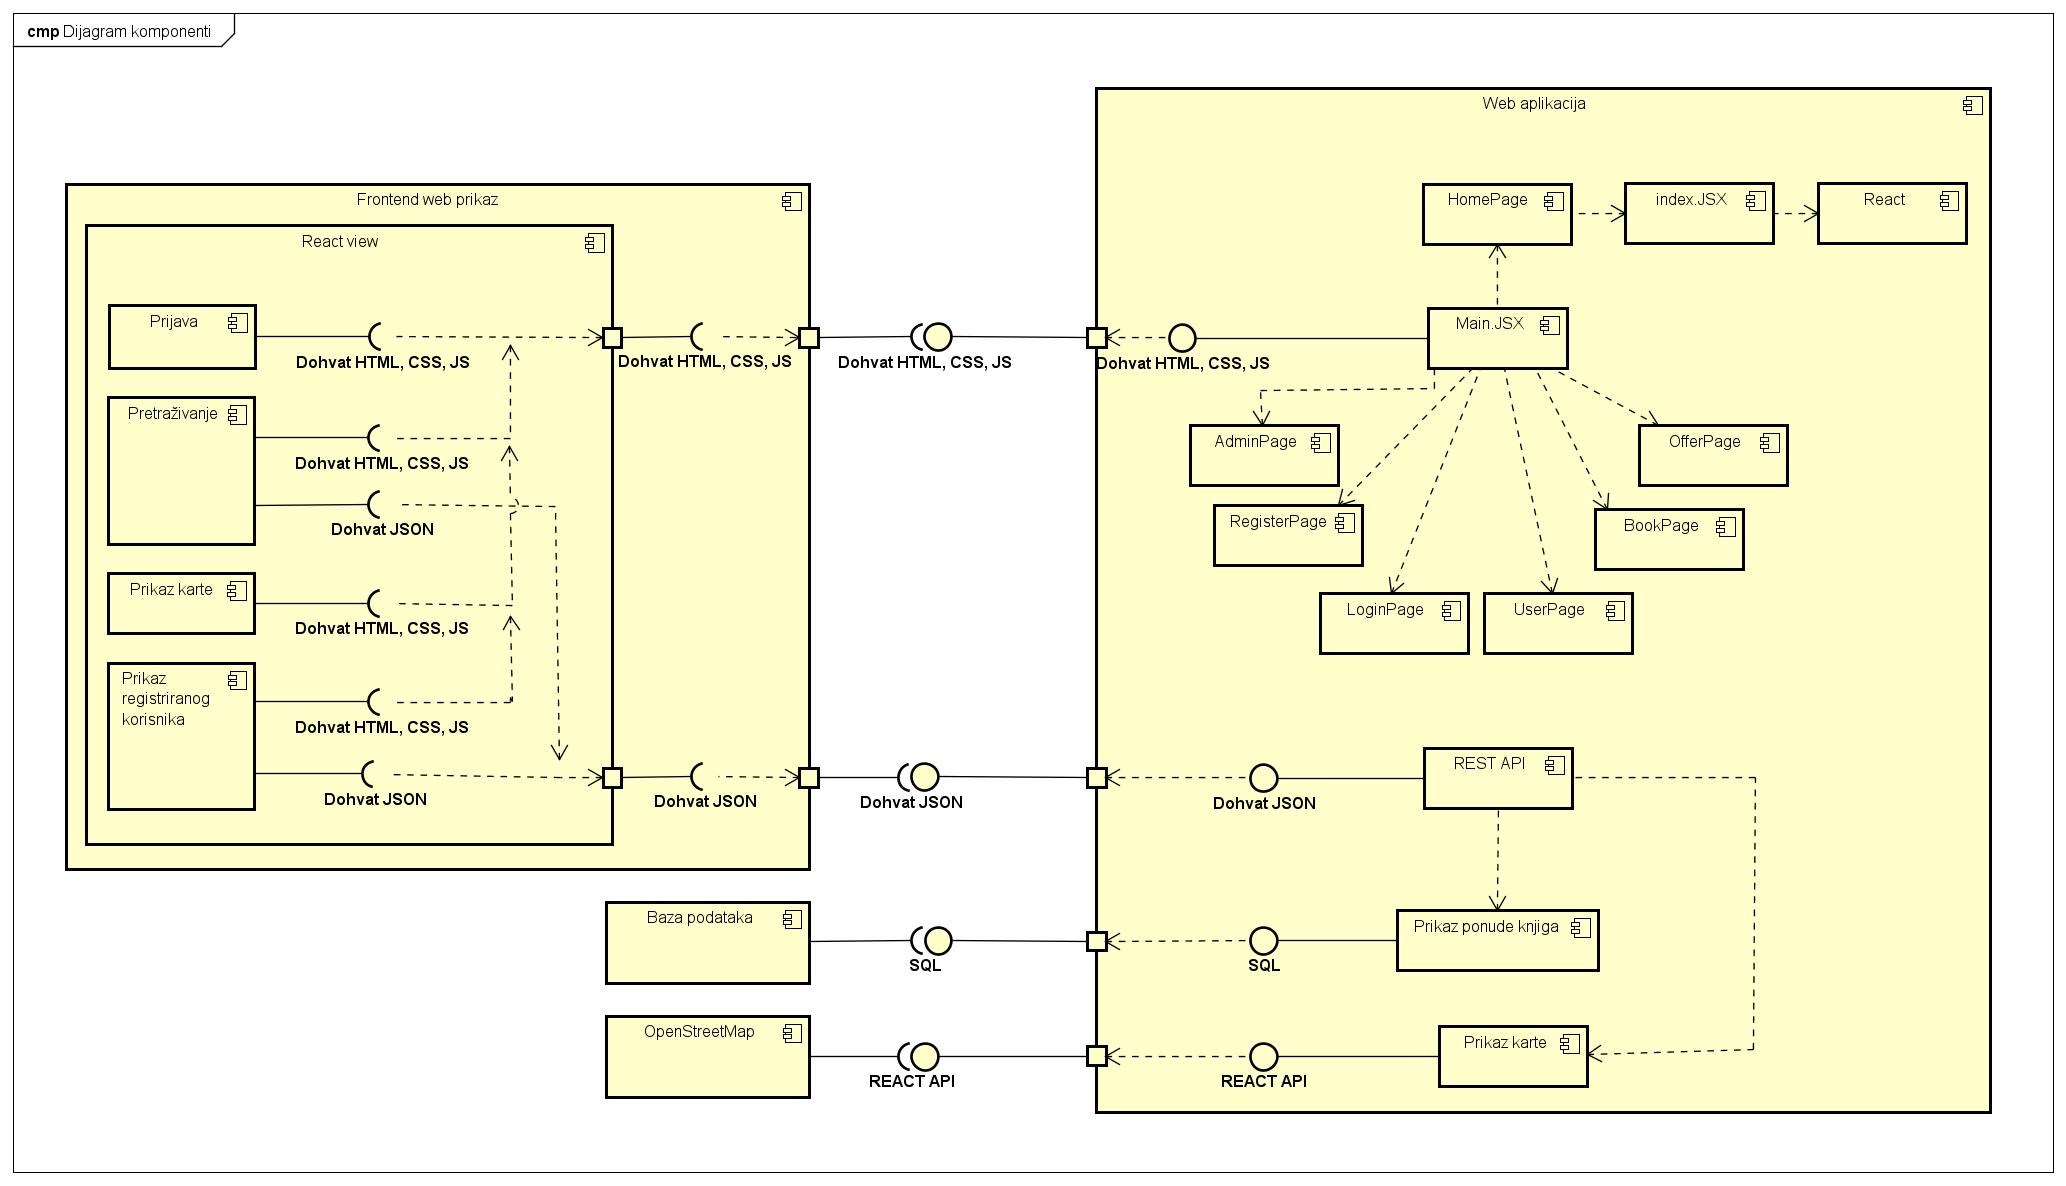
\includegraphics[width=\textwidth]{dijagrami/Dijagram komponenti.PNG} %veličina u odnosu na širinu linije
				\centering
				\caption{Dijagram komponenti }
				\label{fig:dijagramkomponenti1}
			\end{figure}
			
			\eject
